\documentclass[12pt]{scrartcl}
\usepackage{graphicx}
\usepackage{float}
\usepackage[figurename=Figure]{caption}
\usepackage{verbatim} % For comments and other
\usepackage{amsmath}  % For math
\usepackage{amssymb}  % For more math
\usepackage{fullpage}
\usepackage{paralist} % paragraph spacing
\usepackage{listings} % For source code
\usepackage{subfig}

\usepackage{enumitem} % useful for itemization
\usepackage{siunitx}  % standardization of si units

\usepackage{tikz,bm} % Useful for drawing plots
\usepackage{tikz-3dplot}

\usepackage{setspace}
\usepackage{geometry}

\geometry{
left=20mm,
top=10mm,
bottom=10mm,
}

\Large


\begin{document}

\onehalfspacing
\newcommand{\current}{June 2023}
\begin{center}
\hrule
\vspace{.4cm}
{\textbf { \large COL334 Computer Networks SEM II 2023-24}}
\end{center}
{
    \begin{center}
        Vatsal Jingar (2020CS50449)\\ Stitiprajna Sahoo (2020CS10394)\\ Tanish Gupta (2020CS10397)\\
        \textbf{Date:} 8 September 2023 \\
        \textbf{Assignment 2: Mimicking distributed file transfer}
    
    \end{center}
{ 
    \hrule
}
}

\section{Introduction}

As a part of this assignment, we learnt about socket programming using TCP. We exploited the mesh network structure (since there were only 4 clients), each client running 4 threads - 1 connecting it to the server, and the remaining 3 for P2P connections. In the remainder of this document, we first describe the different modules of our code structure, and then look into each one deeply using its C++ implementation. We include relevant details and the logic along with different code segments. Finally, we present some analysis reports.

\section{Implementation in C++ (g++ 10.4)}
\begin{enumerate}
    \item \textbf{clientburst.cpp}\\
    This file contains the code logic for receiving packets continuously from the server.
    \item \textbf{clientrecv.cpp}\\
    Client will receive the packets continuously from its peer client (P2P connections). Recall that all these connections (and the one with server) run on different ports with the help of different threads.
    \item \textbf{clientbroadcast.cpp}\\
    Client will broadcast the packets to its peer clients continuously.
    \item \textbf{controller.cpp}\\
    Controls the logic of the client. It can be thought of as an entity that binds together different threads. For example, Every client will keep count of how many lines it has received. When it is L = 1000, it will communicate it with the main thread.
    \item \textbf{driver.cpp}\\
    Specific implementation is included in subsequent sections. In short, Every client can run this file with their respective IP addresses (which have been defined in constants.h header file to maintain modularity).
    \item \textbf{constants.h}\\
    All the constants including Number of clients, Port Numbers, IP Addresses of clients are defined here.
\end{enumerate}



\subsection{Code Structure}
\begin{center}
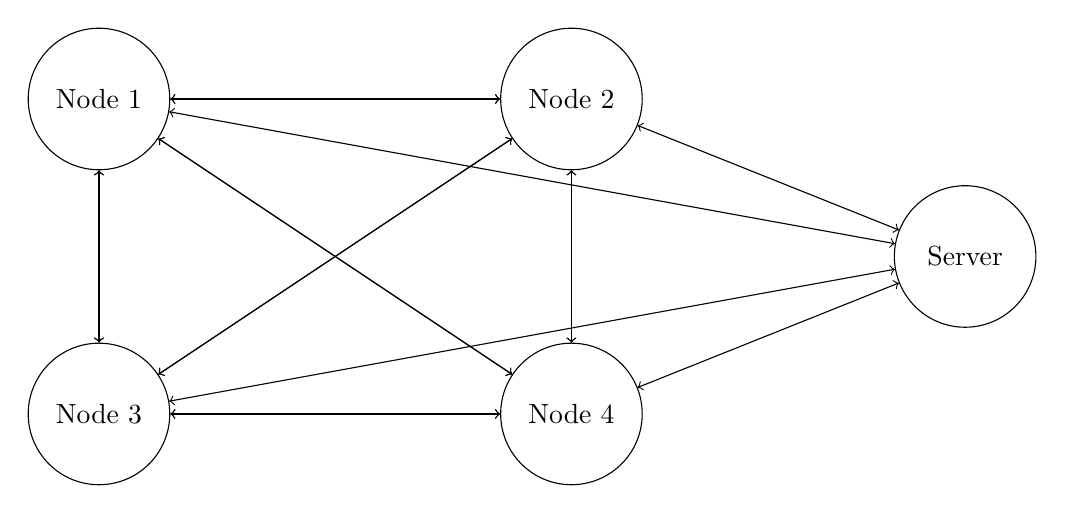
\begin{tikzpicture}
    % Draw central server
    \node[draw, circle, text width=1.5cm, align=center] (server) at (8, 0) {Server};
    
    % Draw nodes
    \node[draw, circle, text width=1.5cm, align=center] (node1) at (-3, 2) {Node 1};
    \node[draw, circle, text width=1.5cm, align=center] (node2) at (3, 2) {Node 2};
    \node[draw, circle, text width=1.5cm, align=center] (node3) at (-3, -2) {Node 3};
    \node[draw, circle, text width=1.5cm, align=center] (node4) at (3, -2) {Node 4};
    
    % Draw communication lines
    \draw[<->] (node1) -- (server);
    \draw[<->] (node2) -- (server);
    \draw[<->] (node3) -- (server);
    \draw[<->] (node4) -- (server);
    
    \draw[<->] (node1) -- (node2);
    \draw[<->] (node1) -- (node3);
    \draw[<->] (node1) -- (node4);
    
    \draw[<->] (node2) -- (node1);
    \draw[<->] (node2) -- (node3);
    \draw[<->] (node2) -- (node4);
    
    \draw[<->] (node3) -- (node1);
    \draw[<->] (node3) -- (node2);
    \draw[<->] (node3) -- (node4);
    
    \draw[<->] (node4) -- (node1);
    \draw[<->] (node4) -- (node2);
    \draw[<->] (node4) -- (node3);
\end{tikzpicture}
\end{center}

% \subsubsection{Central Struct : "Client_data"}
\textbf{1. Central Struct : "Client\_data"}\\
This struct contains all the data that is required for the client to communicate with peers. This is the common data structure that is shared among all the threads of a single client. It contains all the logic - including receiving lines and communicating them to other peers. \\
\begin{verbatim}
    struct Client_data{
        bool received[L];
        string data[L];
        bool complete;
        int port[N];
        const char *ips[N];
        vector<int> broadcast;
        int clientid;
    };
\end{verbatim}
\begin{itemize}
    \item \textbf{received[L]} : This array contains the information about which lines have been received (both from the server and other clients). Here, L is the total number of lines which has been predefined in the constants.h file. 
    \item \textbf{data[L]} : This array contains the data of the lines that have been received.
    \item \textbf{complete} : This variable tells whether the client has received all the lines or not. Precisely, "complete" is true if and only if all elements of "received" array are true.
    \item \textbf{port[N]} : This array contains the port numbers of the peers (the port where we need to send the line).
    \item \textbf{ips[N]} : This array contains the IP addresses of the peers.
    \item \textbf{broadcast} : This vector contains the information about which lines are yet to be broadcasted. Initially, "broadcast" was a boolean array which held the information about each line if it was broadcasted yet or not. As the part of an optimzation, we now only push those line numbers to this vector, which are to be sent next. (Note that, this is similar to a queue, but NOT a queue. Since different threads need to cooperate and send the data to different clients at different speeds, we can not pop from the queue. Thus, we maintain a separate index for each P2P connection - which contains the index upto which the data has been sent).
    \item \textbf{clientid} : This variable contains the id of "this" client - Every client is assigned a unique ID.
\end{itemize}

\textbf{2. Driver.cpp}\\
\begin{verbatim}
    int main(){
        // assert((int)client_ips.size() == N);
        vector<pthread_t> clients(N);
        vector<struct Client_data> args;
        vector<int> ports;
        for(int i = 0; i < N;i++){
            struct Client_data temp;
            args.push_back(temp);
            args[i].complete = 0;
            args[i].clientid = i;
            args[i].ips[i] = client_ips[i];
        }
        client((void*) &args[client_id]);
        cout << "Completed Session\n";
        return 0;
    }
\end{verbatim}
This file is the driver for starting the client. It calls the client function with certain parameters including client ID and IP address. (Notice that the client\_ips array is defined in the constants.h file)\\
\\
\textbf{3. Client.cpp}\\

This file is the first entry point for each client. There are a number of steps that need to be performed here.

\textbf{3.1 Client Data Initialization}
\begin{verbatim}
    void* client(void* arg){
        struct Client_data* args = (struct Client_data*) arg;
        for (int i = 0; i < L; i++) {
            args->received[i] = false;
            args->data[i] = "0";
        }
        args->complete = 0;
    }
\end{verbatim}
All the clients will initialize their struct attributes including received array and data array. Each client will also set the "complete" variable to false.\\

\textbf{3.2 Client Sub modules}:
\begin{verbatim}
    pthread_t clientburster, clientrecver, clientcontroller, clientbroadcaster;
    
    pthread_create(&clientburster, NULL, clientburst, (void*) &(*args));
    pthread_create(&clientrecver, NULL, clientrecv, (void*) &(*args));
    pthread_create(&clientbroadcaster, NULL, clientbroadcast, (void*) &(*args));
    pthread_create(&clientcontroller, NULL, controller, (void*) &(*args));

    pthread_join(clientburster, NULL);
    pthread_join(clientrecver,NULL);
    pthread_join(clientbroadcaster, NULL);
    pthread_join(clientcontroller, NULL);
\end{verbatim}
This file creates 4 submodules for the client i.e. runs 4 different functionalities on 4 different threads. \\

\textbf{3.2.1 Clientburst}\\
This thread will continuously receive the packets from the server.\\

\textbf{3.2.2 Clientrecv}\\
This thread will continuously receive the packets from the peer client.\\

\textbf{3.2.3 Clientbroadcast}\\
This thread will continuously broadcast the packets to the peer clients.\\

\textbf{3.2.4 Controller}\\
This thread will continuously check whether the client has received all the packets or not, and perform overall control functions.\\

\textbf{4. Clientburst.cpp}\\

The crux of this file, as mentioned before, is to continously receive data from the server. \\

\textbf{4.1 Creation and Connecting Socket with Server}

The following is some boilerplate code needed to connect with the server.

\begin{verbatim}
        struct Client_data *needdata = (struct Client_data*) args;
        int status, client_fd;
        struct sockaddr_in serv_addr;
        const char *sendline = "SENDLINE\n";
        char buffer[BUFFER_SIZE];
        if ((client_fd = socket(AF_INET, SOCK_STREAM, 0)) < 0){
            printf("\nSocket creation error \n");
            RETURN(2);
        }
        serv_addr.sin_family = AF_INET;
        serv_addr.sin_port = htons(PORT);
        if (inet_pton(AF_INET, serverIP, &serv_addr.sin_addr) <= 0){
            printf("\nInvalid address/ Address not supported \n");
            RETURN(2);
        }
\end{verbatim}

A quick note - "RETURN" is a macro defined in the constants.h file. \\

\textbf{4.2 Sending SENDLINE to Server}
\begin{verbatim}
        while (!needdata->complete) {
            if(send(client_fd, sendline, strlen(sendline), 0) < 0){
                perror("send");
                continue;
            }
\end{verbatim}

So, while the complete data is not received, we send the SENDLINE message to the server. \\

\textbf{4.3 Receiving the Data from Server}
\begin{verbatim}
    while(count < 2){
        int x = recv(client_fd, buffer, BUFFER_SIZE, 0);
        if(x < 0){
            perror("recv");
            continue;
        }
        for(int i = 0; i < x; i++){
            if(buffer[i] == '\n') count++;
            mystring += buffer[i];
            if(count == 2) break;
        }
    }
\end{verbatim}

Here, count keeps the track of number of linebreaks that have been seen yet. While we do not get 2 linebreaks, we keep on "recv" the data from the server. This happens because the socket file can only send a fragment of the data in the buffer. Thus, we need to read it in a while loop.\\ 

\textbf{4.4 Parsing the Data}
\begin{verbatim}
    while (i < (int)mystring.size() && mystring[i] != '\n'){
        line_num = 10 * line_num + (mystring[i] - '0');
        i++;
    }
    if (line_num >= 0 && line_num < L && !needdata->received[line_num]){
        string data = "";
        for (int j = i + 1; j < (int)mystring.length(); j++){
            data += mystring[j];
            if(mystring[j] == '\n') break;
        }
        cnt++;
        // cout << line_num << endl;
        needdata->data[line_num] = data;
        needdata->received[line_num] = true;
        needdata->broadcast.push_back(line_num);
    }
\end{verbatim}\\

The number before the first line-break contains the line number, and the data after that is the line data. This part of code just parses the data received from the server. \\ 

\textbf{5. Clientrecv.cpp}\\

\textbf{Logic:}
\begin{itemize}
    \item Every client will create a socket (unique to connect with each other client) and bind it to one of its port. Then it will start receiving for the packets from its peer clients. When it receives the packets, it will parse the data and store it in its data array. It will also update the "received" array. 
    \item As a part of an optimization, rather than sending one line at a time, we send multiple lines at once. Thus, the data which would be received from the peer client would look like \[\mbox{"line\_number\textbackslash n line\_data\textbackslash n...line\_number\textbackslash n line\_data\textbackslash n"}\]\\ 
    For every client, we will have N sockets which will try to connect to the peer clients. The port number of the socket to which it will try to connect will be a function of client id of peer. We will maintain a vector of sockets which will be used to communicate with the peer clients.
    \item As the data received from peer is of the complex form, clientrecv will need to parse the data.
\end{itemize}

\textbf{Converting Data into the required form}
\begin{verbatim}
    reading = "";
    while(count < 2){
        int x = recv(sock, buff, BUFFER_SIZE, 0);
        if(x < 0){
            perror("recv");
            continue;
        }
        for(int i = 0; i < x; i++){
            if(buff[i] == '\n') {
                count++;
            }
            else{
                count = 0;
            }
            reading += buff[i];
            if(count == 2){
                break;
            }
        }
    }
\end{verbatim}
\par We create a string reading. We keep on appending the data to the string reading until we encounter two line breaks, after which we break the loop. To indicate the end of data, we append one extra line break at the end. Thus, if two consecutive linebreaks are received, we get out of the overall loop.\\

We know that the underlying protocol TCP is reliable but it uses streams. Hence it could happen that data written in kernel socket file is not complete and received in chunks. So to ensure that we have recevied all the data, we will keep writing on the client buffer until we encounter two consecutive line breaks.\\

For the remaining data parsing, we do it the same way as it was done in clientburst.\\

\textbf{6. Clientbroadcast.cpp}\\

\textbf{Logic:} \\

\par Initially, we had implemented a boolean array (of length L) which stored true if we had broadcasted that line, and false otherwise. (So, we had to send a line, if received[i] was true but broadcasted[i] was false). With this approach, we sent only one line at a time, and looped over the entire array to check which line to broadcast next, which takes O(L) time everytime. \\

To optimize this, we created a queue of lines which are yet to be broadcasted (So, this queue contains only the line numbers which are received from the server, but not yet broadcasted i.e. Just push to the queue as soon as a line is received from the server). Whenever we will see that there is some data to broadcast (could be any number of lines), we begin to collect this data to be sent. To achieve the functionality of iterating over queue, we have implemented it using a C++ vector. One other reason to use a vector is that, we do not want to pop the data from the queue, since all the threads (each thread sending to a different client) do not work on same speed. If we pop the data, it might not be available for other threads (Recall that this struct is shared among all threads). We will iterate over the queue till the length we saw and create a string temp which will contain the data in the form of \[\mbox{"line\_number\textbackslash n line\_data\textbackslash n...line\_number\textbackslash n line\_data\textbackslash n\textbackslash n"}\]\\

(Recall the two line breaks at the end of the data stream). 

\begin{verbatim}
    if(data->broadcast_idx < (int)data->needed_data->broadcast.size()){
        string temp = "";
        int lengthofvector = data->needed_data->broadcast.size();
        while(data->broadcast_idx  < lengthofvector){
            int i = data->needed_data->broadcast[data->broadcast_idx];
            data->broadcast_idx++;
            temp += (to_string(i) + "\n" + data->needed_data->data[i]);
        }
        temp += "\n";
        const char *temp1 = temp.c_str();
        if(send(sock, temp1, strlen(temp1), MSG_NOSIGNAL) < 0){
            perror("send");
            continue;
        }
        data->sent = true;
    }
\end{verbatim}

\textbf{7. Calculating the peer ports}

\begin{itemize}
    \item Every client will create N sockets for peers. One socket will always be empty. All the other sockets would be used to communicate with other clients.
    \item The ports of the sockets would be calculated as follows: $$BASE\_PORT + (this\rightarrow clientid * N) + i;$$
    i is the client\_id of the other client, and N is the total number of clients.
    \item Every client will connect to the ports:  $$BASE\_PORT + (i * N) + this\rightarrow clientid;$$
    \item This will ensure that every client will connect to every other client.
\end{itemize}
\begin{center}
    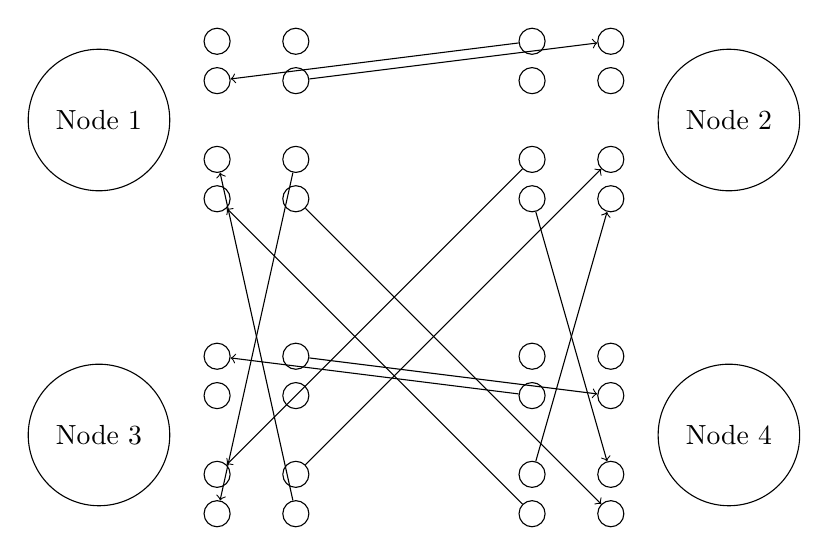
\begin{tikzpicture}
        % Draw central server
        % \node[draw, circle, text width=1.5cm, align=center] (server) at (8, 0) {Server};
        
        % Draw nodes
        
            \node[draw, circle, align=center, minimum size = 0.4] (port1n1) at (-1.5, 3) {};
            \node[draw, circle, align=center, minimum size = 0.4] (port2n1) at (-1.5, 2.5) {};
            \node[draw, circle, align=center, minimum size = 0.4] (port3n1) at (-1.5, 1.5) {};
            \node[draw, circle, align=center, minimum size = 0.4] (port4n1) at (-1.5, 1) {};
            \node[draw, circle, align=center, minimum size = 0.4] (port1n2) at (3.5, 3) {};
            \node[draw, circle, align=center, minimum size = 0.4] (port2n2) at (3.5, 2.5) {};
            \node[draw, circle, align=center, minimum size = 0.4] (port3n2) at (3.5, 1.5) {};
            \node[draw, circle, align=center, minimum size = 0.4] (port4n2) at (3.5, 1) {};
            \node[draw, circle, align=center, minimum size = 0.4] (port1n3) at (-1.5, -3) {};
            \node[draw, circle, align=center, minimum size = 0.4] (port2n3) at (-1.5, -2.5) {};
            \node[draw, circle, align=center, minimum size = 0.4] (port3n3) at (-1.5, -1.5) {};
            \node[draw, circle, align=center, minimum size = 0.4] (port4n3) at (-1.5, -1) {};
            \node[draw, circle, align=center, minimum size = 0.4] (port1n4) at (3.5, -3) {};
            \node[draw, circle, align=center, minimum size = 0.4] (port2n4) at (3.5, -2.5) {};
            \node[draw, circle, align=center, minimum size = 0.4] (port3n4) at (3.5, -1.5) {};
            \node[draw, circle, align=center, minimum size = 0.4] (port4n4) at (3.5, -1) {};


            \node[draw, circle, align=center, minimum size = 0.4] (rport1n1) at (-0.5, 3) {};
            \node[draw, circle, align=center, minimum size = 0.4] (rport2n1) at (-0.5, 2.5) {};
            \node[draw, circle, align=center, minimum size = 0.4] (rport3n1) at (-0.5, 1.5) {};
            \node[draw, circle, align=center, minimum size = 0.4] (rport4n1) at (-0.5, 1) {};
            \node[draw, circle, align=center, minimum size = 0.4] (rport1n2) at (2.5, 3) {};
            \node[draw, circle, align=center, minimum size = 0.4] (rport2n2) at (2.5, 2.5) {};
            \node[draw, circle, align=center, minimum size = 0.4] (rport3n2) at (2.5, 1.5) {};
            \node[draw, circle, align=center, minimum size = 0.4] (rport4n2) at (2.5, 1) {};
            \node[draw, circle, align=center, minimum size = 0.4] (rport1n3) at (-0.5, -3) {};
            \node[draw, circle, align=center, minimum size = 0.4] (rport2n3) at (-0.5, -2.5) {};
            \node[draw, circle, align=center, minimum size = 0.4] (rport3n3) at (-0.5, -1.5) {};
            \node[draw, circle, align=center, minimum size = 0.4] (rport4n3) at (-0.5, -1) {};
            \node[draw, circle, align=center, minimum size = 0.4] (rport1n4) at (2.5, -3) {};
            \node[draw, circle, align=center, minimum size = 0.4] (rport2n4) at (2.5, -2.5) {};
            \node[draw, circle, align=center, minimum size = 0.4] (rport3n4) at (2.5, -1.5) {};
            \node[draw, circle, align=center, minimum size = 0.4] (rport4n4) at (2.5, -1) {};
        \node[draw, circle, text width=1.5cm, align=center] (node1) at (-3, 2) {Node 1};
        \node[draw, circle, text width=1.5cm, align=center] (node2) at (5, 2) {Node 2};
        \node[draw, circle, text width=1.5cm, align=center] (node3) at (-3, -2) {Node 3};
        \node[draw, circle, text width=1.5cm, align=center] (node4) at (5, -2) {Node 4};
        
        % Draw communication lines
        \draw[<-] (port2n1) -- (rport1n2);
        \draw[<-] (port3n1) -- (rport1n3);
        \draw[<-] (port4n1) -- (rport1n4);

        \draw[<-] (port1n4) -- (rport4n1);
        \draw[<-] (port2n4) -- (rport4n2);
        \draw[<-] (port3n4) -- (rport4n3);

        \draw[<-] (port1n3) -- (rport3n1);
        \draw[<-] (port2n3) -- (rport3n2);
        \draw[<-] (port4n3) -- (rport3n4);

        \draw[<-] (port1n2) -- (rport2n1);
        \draw[<-] (port3n2) -- (rport2n3);
        \draw[<-] (port4n2) -- (rport2n4);
        % \draw[<->] (node2) -- (server);
        % \draw[<->] (node3) -- (server);
        % \draw[<->] (node4) -- (server);
        
        % \draw[<->] (node1) -- (node2);
        % \draw[<->] (node1) -- (node3);
        % \draw[<->] (node1) -- (node4);
        
        % \draw[<->] (node2) -- (node1);
        % \draw[<->] (node2) -- (node3);
        % \draw[<->] (node2) -- (node4);
        
        % \draw[<->] (node3) -- (node1);
        % \draw[<->] (node3) -- (node2);
        % \draw[<->] (node3) -- (node4);
        
        % \draw[<->] (node4) -- (node1);
        % \draw[<->] (node4) -- (node2);
        % \draw[<->] (node4) -- (node3);
    \end{tikzpicture}
    \end{center}
\begin{itemize}
    \item Figure shows the way in which Clients are connecting each other, Left Small circles represent Listening ports and Right Small circles represent receiving ports
    \item Every Client can calculate its reserved port by mathematical equation presented above. 
    \item It could be observed that every client would have one pair of port empty.
    \item For the pictorial view of mathematical equation, this is what really happening. For efficient utilization of ports, we have not made sockets for port$(==)$clientid.
\end{itemize}

\subsection{Fault Resistent Design and Implementation}
\begin{itemize}
    \item \textbf{Recovery from Suddenly Disconnected Client} : There could be situations of deadlocks, where receiving keep trying to receive data from the client which is not sending any data. To avoid this, we used the return value of recv() which 0 when peer connection breaks. In this we are assuming that the peer has broadcasted all the data it has, and now it is Disconnected. This is always the case in our design as we are using TCP which is a reliable protocol. So if a peer suddenly breaks a connection, we will also close the socket, Whenever recv returns 0.
    \item \textbf{Consistency between Data sent and received} : TCP is a stream protocol, Whenever we use send function, it just writes it in the Kernel buffer, where Kernel TCP will send it according to fragment size of underlying protocols. Due to which at receiving side, recv can give us data in chunks. To avoid this, we have used two consecutive line breaks to indicate the end of data. So we will keep on receiving data until we encounter two consecutive line breaks. This will ensure that we have received all the data sent by the peer.
    \item \textbf{Consistency of Data} : We have used seperate ports for receving and sending for each pair of client, this will keep the data from different clients seperate. Also we have used seperate sockets for each pair of client, this will ensure that data from different clients will not mix up.
    \item \textbf{Fault Recovery} : If any of the clients suddenly dies due to any reasons, our implementation could make connection with that cleint again. This is because we have used seperate sockets for each pair of client. So if any of the cleint dies, then also other reserved sockets would be listening for it, till they are not closed.
    \item \textbf{Sending Data after submission} : For reducing latency overall of the system, any client who receives all the data and had submiited its file, will not complete until it broadcasts all the data it has.
    \item \textbf{Reusing Ports} : It is possible that the port we are assigning any thread could be in a zombie state with any other process, in which case, we are calling setsockopt, which we will help in reusing such sockets, other, it would not connect with other peers.
\end{itemize}

\section{Analysis}

We have tested the code extensively for N = 1, 2, 3 and 4 clients. One of the important realizations that we made was that the variance in the total time taken was significant, perhaps due to the server load. On the last date of submission, the server load seemed to be too high. Nevertheless, we present time from one of the runs here for each N, and a range of values for time taken that we experienced. 

\subsection{N = 1}

\begin{figure}[H]
    \centering
    \includegraphics[width=0.8\textwidth]{images/latency_n_1.png}
    \caption{Time taken when only 1 client}
    \label{fig:my_label}
\end{figure}

As expected, initially the number of unique lines received is too high, and hence, the slope of the graph is very small. With time, the probability of receiving a unique line decreases, and hence, it takes longer to receive more unique lines. As can be seen from the graph, approx. 80\% of the lines was received in 15 seconds, and 90\% of the lines in around 25 seconds. The last 100 lines took almost 50 seconds to be received.

The range of values for time taken were between 60 seconds and 80 seconds.

\subsection{N = 2}

\begin{figure}[H]
    \centering
    \includegraphics[width=0.8\textwidth]{images/latency_n_2.png}
    \caption{Time taken with 2 clients}
    \label{fig:my_label}
\end{figure}

The overall execution time for N=2 clients is around 30 seconds. This is a significant improvement over N=1. 

The range of values for time taken were between 30 seconds and 35 seconds.

\subsection{N = 3}

\begin{figure}[H]
    \centering
    \includegraphics[width=0.8\textwidth]{images/latency_n_3.png}
    \caption{Time taken with 3 clients}
    \label{fig:my_label}
\end{figure}

The range of values for time taken for N = 3 were between 22 seconds and 28 seconds.

\subsection{N = 4}

\begin{figure}[H]
    \centering
    \includegraphics[width=0.8\textwidth]{images/latency_n_4.png}
    \caption{Time taken with 4 clients}
    \label{fig:my_label}
\end{figure}

The range of values for time taken for N = 4 were between 15 seconds and 22 seconds.

\subsection{Relation between Number of Clients and Time}

As can be seen in the above graphs, the time decreases as more nodes are added. As a part of our analysis, we also printed the number of lines for each client, that were received from the server, and those that were received from other clients. The results were nice - for N clients, as expected almost \(\frac{1000}{N}\) lines were received by each client from the server. This uniform distribution helps in good speed. \\

\begin{figure}[H]
    \centering
    \includegraphics[width=0.8\textwidth]{images/download.png}
    \caption{Time taken vs Number of clients}
    \label{fig:my_label}
\end{figure}


We even tested with N clients, when only some x \((< N)\) receives the lines from the server, and others just receive lines from other clients after those x clients have received all the lines. This was done to check if memory limits are violated and the speed of P2P connections. It worked correctly, and the speed was very fast (in less than a second!). 



\end{document}